\section{Analyse de l'existant}
\label{chap:analyse_existant}
% [Votre texte ici]
%\lipsum[1]

\subsection{Partie 1}
\label{sec:existant_partie1}
% [Votre texte ici]
%\lipsum[2]
\subsubsection{Sous-partie 1}
\label{ssec:existant_partie1_sous1}
% Contenu
% [Votre texte ici]
%\lipsum[3]

\subsubsection{Sous-partie 2}
\label{ssec:existant_partie1_sous2}
% Contenu
% [Votre texte ici]
%\lipsum[4-5]

\subsection{Partie 2}
\label{sec:existant_partie2}
% Contenu
% [Votre texte ici]
%\lipsum[6]

\begin{figure}[h!]
    \centering
    % Pour inclure une image, utilisez la commande \includegraphics.
    % 'width=\linewidth' ajuste la largeur de l'image à la largeur de la ligne de texte.
    % Vous pouvez utiliser des valeurs absolues (ex: width=10cm) ou relatives.
    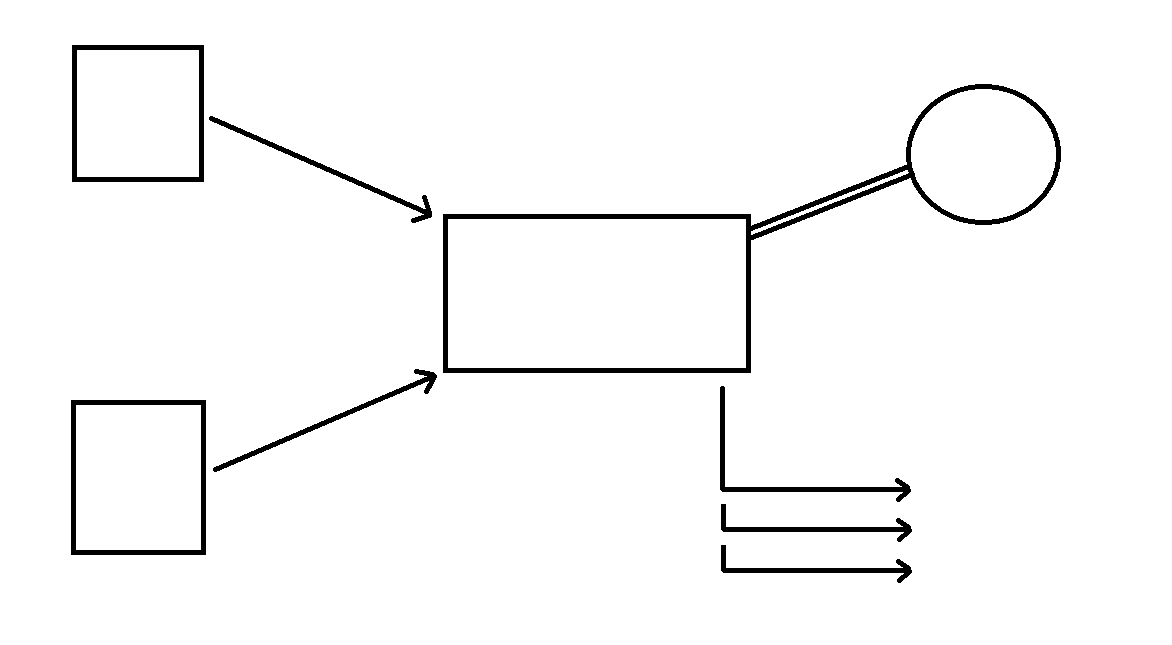
\includegraphics[width=0.8\linewidth]{figs/schema.png}
    \caption{Schéma fonctionnel de la solution existante.}
    \label{fig:schema_existant}
\end{figure}

\subsection{Bilan récapitulatif}
\label{sec:bilan_recap}
% Voici un exemple de tableau comparatif. Le paquet 'booktabs' est utilisé pour les lignes.
\begin{table}[H]
\centering
\caption{Comparaison des technologies d'analyse de données.}
\label{tab:tech_comparison}
\begin{tabular}{lccc}
\toprule
\textbf{Technologie} & \textbf{Type} & \textbf{Avantages} & \textbf{Inconvénients} \\
\midrule
Solution A & Cloud & Scalabilité, Maintenance réduite & Coût, Dépendance \\
Solution B & On-premise & Contrôle, Sécurité & Coût initial, Maintenance \\
Solution C & Hybride & Flexibilité & Complexité \\
\bottomrule
\end{tabular}
\end{table}

% [Votre texte ici]
%\lipsum[7] 